\documentclass[conference]{IEEEtran}
%\IEEEoverridecommandlockouts
% The preceding line is only needed to identify funding in the first footnote. If that is unneeded, please comment it out.
\usepackage{cite}
\usepackage{amsmath,amssymb,amsfonts}
\usepackage{algorithmic}
\usepackage{graphicx}
\graphicspath{ {images/} }
\usepackage{textcomp}
\usepackage{xcolor}
\usepackage{caption}
\def\BibTeX{{\rm B\kern-.05em{\sc i\kern-.025em b}\kern-.08em
    T\kern-.1667em\lower.7ex\hbox{E}\kern-.125emX}}
\begin{document}

\title{Recurrent Neural Networks for object detection}

<<<<<<< HEAD
\author{\IEEEauthorblockN{Bin Qassim Ahmad}
\IEEEauthorblockA{\textit{Technical University of Munich} \\
\textit{Department of Informatics}\\
Munich, Germany \\
ahmad.qasim@tum.de }
\and
\IEEEauthorblockN{Pettirsch Arnd}
\IEEEauthorblockA{\textit{Technical University of Munich} \\
\textit{Department of Informatics}\\
Munich, Germany \\
a.pettirsch@outlook.de}
}

\maketitle

\begin{abstract}
ToDo
\end{abstract}

\begin{IEEEkeywords}
TBD.
\end{IEEEkeywords}

\section{Introduction}

\subsection{Image and Video Object Detection in general}
\begin{itemize}
	\item Image object detection history.
	\begin{itemize}
		\item Bayesian methods before deep learning
		\item ImageNet challenge and VID [15]
		\item Deep Learning and AlexNet [16]
	\end{itemize}
	\item Single stage and 2-stage image object detectors.
	\begin{itemize}
		\item A two-stage pipeline firstly generates region proposals, which are then classified and refined. [17]
		\item A single-stage method is often more efficient but less accurate. Directly regress on bounding boxes and classes. [18], [19]
	\end{itemize}
	\item Why is video object detection harder?
	\begin{itemize}
		\item Large size
		\item Motion blur
		\item Quality of the dataset
		\item Partial occlusion
		\item Unconventional Poses
	\end{itemize}
\end{itemize}

\subsection{Recurrent Neural Networks in general}
\subsubsection{Delimitation to non-recurrent Neural Networks} 
Non-recurrent Neural Networks process on single inputs. In the field of image classification this could be for example a single image. \\
Recurrent Neural Networks process on sequences of date. In the field of classification those sequences consist often multiple frames. Recurrent Neural Network's core concept to enable the sequence processing is parameter sharing across different parts of a model. Parameter sharing can be reached by cycles in the architecture. \textbf{[?]} \newline

\subsubsection{Common Types of Recurent Neural Networks}
Most of the paper which are described in this work use two pretty common approaches of Recurrent Neural Networks. The first one are LSTMs, first mentioned in \textbf{[?]} in 1991. The key of LSTMs is the inner cell state. LSTMs consist of four layers. Those four layers are able to remove or add information to the inner cell state. \textbf{[?]} \newline

The second type of Recurrent Neural Networks is Gated Recurrent Units (GRUs). The main difference to LSTMs is, that those GRUs consist out of a single gated unit which can simultaneously control the forgetting factor and decide to update the inner cell state. \textbf{[?]}

\section{Feature-based Video Object Detection}

\subsection{Definition}
First, we want to introduce feature-based Video Object Detection methods. As defined, for example, in \textbf{[?]} feature-based Video Object Detection methods fuse detectors which integrate features from multiple frames into their video detection. In most of our papers those detectors use recurrent units to integrate the visual features from different frames.  

\subsection{Recurrent Multi-frame Single Shot Detector for Video Object Detection}
Broad, Jones and Lee have in \textbf{[?]} and \textbf{[?]} the idea to insert a fusion-layer into a classical Single Shot Detector (SSD) meta-architecture. Based on this idea they research in two main fields: On the one hand, they investigate different fusion methods and on the other hand they try several SSD meta-architectures. The final architecture is shown in \textbf{Fig. 1} \newline

SSDs is generally consist of two main components. First, an so called Feature Extractor which consist of convolutional and pooling layers. As an input the feature extractor gets an image and it outputs feature-maps. The other component is an Detection head which consists of convolutional layers and creates bounding boxes and class probabilities out of the feature maps created by the feature extractor. \newline

As mentioned above Broad, Jones and Lee have the idea to insert a fusion layer in between those two components. As fusion techniques they test simple element-wise operations (e.g.: add or max), simple concatenations of features maps and recurrent layers. Their experiments show that the recurrent layers perform best. Element-wise operations do not lead to an improvement in the mAP. And concatenations just add another depth to the network, which increases the mAP slightly.Only the Recurrent Units add new parameters, to learn temporal context, to the Network. In addition, they observe that recurrent units do not slow down the computational speed significantly. The state of the art SSD, which is used to test the different fusion techniques performs on 55 fps the recurrent one on 50 fps. As a recurrent unit they use GRU because they observ that the results were similar to the results when they use LSTMs but the GRUs perform faster. \newline

In addition to the investigation on the type of fusion layer, Broad, Jones and Lee test different types of SSDs as a baseline for their architecture. They find out that for all baseline SSDs the mAP was higher in comparison to the non-recurrent models. The mAP increase by 2.7 to 5 percent on KITTI dataset. The best results is made with SequeezeNet+ as a baseline SSD network. \newline

Unfortunately, there is only a little information on the training of the Recurrent Multi-frame Single Shot Detector. They use the SequeezeNet Training strategies and a pre-trained version of the baseline SSD. Finally, they use the SequezzeNet fine tuning strategy to train the whole network afterwards. \newline

\textbf{Figure 1} 

\subsection{Mobile Video Object Detection with Temporally Aware Feature Maps}
Liu and Zhu have the goal to design a video object detection architecture, which can run real-time on low-powered mobile and embedded devices. The key of their method is to combine convolutional layers with convolutional LSTMs. On this core idea they do some further research. They test the benefit from adding an LSTM into the baseline SSD, different types of Recurrent Layers (LSTM, GRU and bottleneck LSTMs), different dimensions of their bottleneck LSTMs and different LSTM placement strategies (Single LSTM placement and multiple LSTM placement)  \newline

In the beginning they simply add one LSTM to their baseline SSDs architecture - MobileNet. They observe that adding the LSTM improves the mAP in comparison to their baseline SSD architecture. Moreover, they investigate that the greatest improve is by adding the LSTM after the 13th convolutional Layer of the SSD. \newline

Afterwards, they compare LSTMs, GRUs and Bottleneck LSTMs as different types of Recurrent units by placing them after the 13th convolutional layer. Bottleneck-LSTMs have been designed by Liu and Zhu to increase the efficiency of LSTMs.  For that purpose they use slightly unusual the ReLU function as activation for the LSTM. Moreover they, compute a so called Bottleneck feature map with less input channel than the originally feature map and feed this map into the LSTM to reduce computational power. They come to the conclusion that Bottleneck-LSTMs are more effective the LSTMs and in the case of a convolutional kernel greater 1x1 even more effective than GRUs while attaining comparable perfomance. \newline

In addition to the bottleneck LSTMs Liu and Zhu extend their network with multipliers. They use $\alpha_{base}$, $\alpha_{ssd}$ and $\alpha_{lstm}$ as multiplier to scale the channel dimension of each layer. During their research they find out that the accuracy of the model remains near constant up to $\alpha_{ssd}= 0.25 \alpha$ which means that the output of each LSTM is one-fourth the size of the input. For the other multipliers they use the values: $\alpha_{base} = \alpha$ and $\alpha_{ssd} = 0.5 \alpha$. \newline

As shown in \textbf{Figure} the final model uses LSTMs after all feature maps, because Liu and Zhu observe that there a slight performance improve by adding LSTMs after every feature map and nearly no change in computational cost. \newline

On the training strategy and the loss function Liu and Zhu do not provide any information.

\subsection{Feature Selective Small Object Detection via Knowledge-based recurrent attentive neural networks}
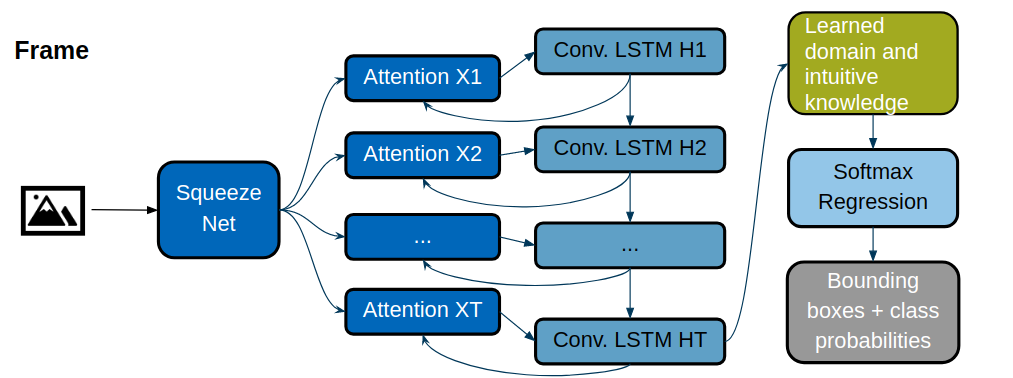
\includegraphics[width=\columnwidth]{KB-RANN-architecture}
\begin{itemize}
	\item Compute feature maps using a modified SqueezeNet architecture.
	\item Propagate the features through a Recurrent Attentive Neural Network, comprised of:
	\begin{itemize}
		\item Attention Mechanism to detect key areas within the feature maps.
		\item Convolutional LSTM for temporal feature propagation.	
	\end{itemize}
	\item Reverse gaussian feature maps are combined with the maps obtained from Conv. LSTM.
	\begin{itemize}
		\item These feature maps are based on learnable mean and covariance terms.
		\item This prior knowledge is derived from the assumption that traffic signs are always located at the bias of the center.

	\end{itemize}
\end{itemize}

\subsection{Looking fast and slow: memory-guided mobile video object detection}
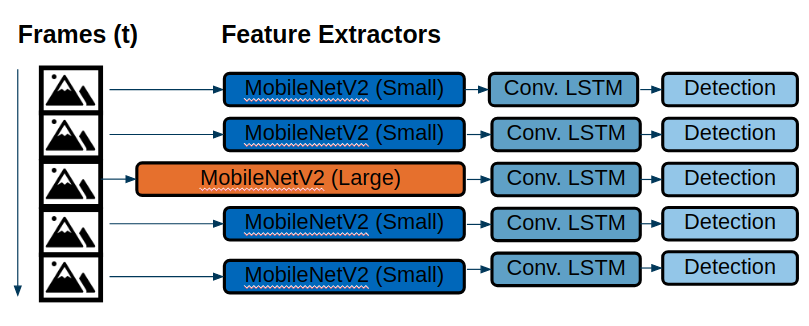
\includegraphics[width=\columnwidth]{looking-fast-and-slow-architecture}
\begin{itemize}
	\item Run multiple feature extractors sequentially or concurrently to obtain feature maps.
	\begin{itemize}
		\item 	The idea is to use small and large feature extractors to optimize performance.
	\end{itemize}
	\item Aggregate and refine these feature maps using convolutional LSTM based memory network.
	\begin{itemize}
		\item To improve speed of LSTM network, add skip connections and LSTM state groups.
	\end{itemize}
	\item Apply SSD-style detection on refined features to obtain classification and bounding boxes.
	\item Use a reinforcement learning based policy for selection of which feature extractor to run.
	\item Large and small frame extractors can run in parallel using asynchronous mode.
\end{itemize}

\subsection{Detect to Track and track to detect}
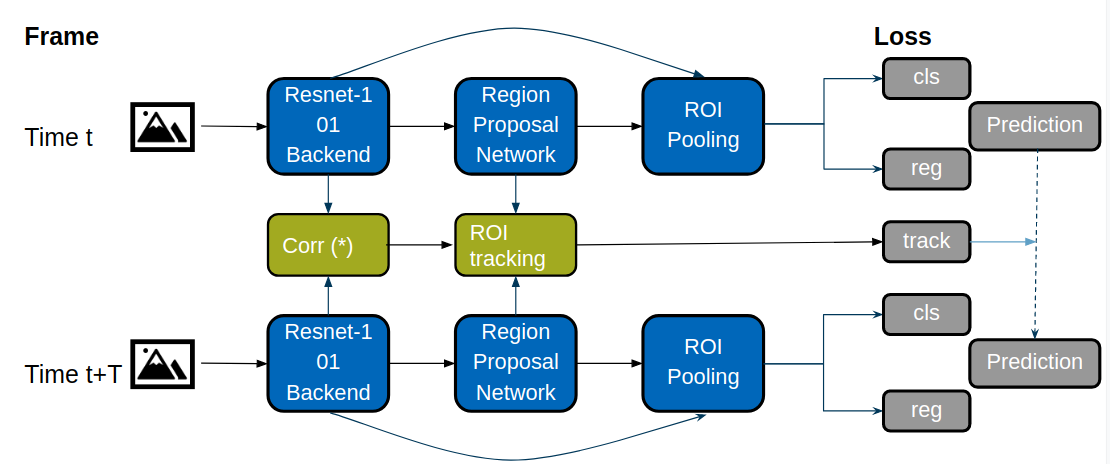
\includegraphics[width=\columnwidth]{D&T-architecture}
\begin{itemize}
	\item Compute Convolutional feature maps using a Resnet-101 architecture.
	\item Use a RPN (region proposal network) to find candidate regions in the frame.
	\item ROI Pooling layer, to classify boxes and refine their coordinates (regression).
	\item Find correlation features between two frames’ feature maps and do ROI tracking.
	\item Due to memory constraints, use tracklets, which are class-based optimal paths in video.

\end{itemize}

\section{Box-Level-based Video Object Detection}

\subsection{Definition}
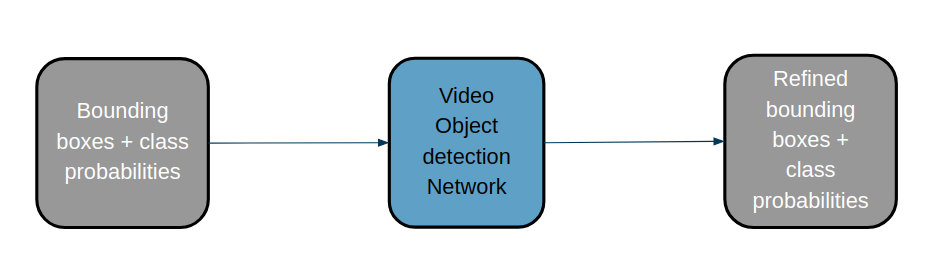
\includegraphics[width=\columnwidth]{box-level-basic}
Bounding Boxes and Class probabilities are fed into the network and are refined temporally and/or spatially.

\subsection{Object Detection from Video Tubelets with Convolutional Neural Networks}
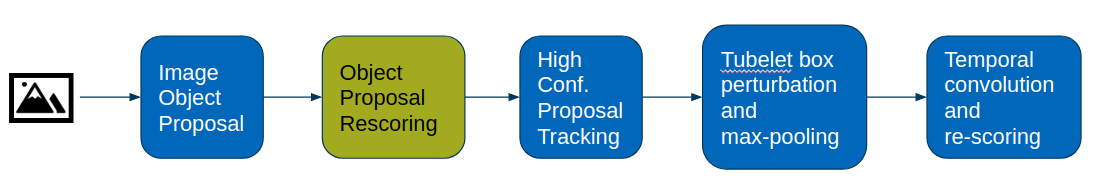
\includegraphics[width=\columnwidth]{video-tubelets-architecture}
\begin{itemize}
	\item Use selective search algorithm to generate around 2000 object proposals on each frame.
	\item Use GoogleNet for feature extraction and then 30 SVMs for 30 VID classes to generate object proposal scores for each object proposal.
	\item Track high confidence targets bi-directionally.
	\item Two kinds of Perturbations:
	\begin{itemize}
		\item The first method is to generate new boxes around each tubelet box on each frame by randomly perturbing the boundaries of the tubelet box.
		\item The second perturbation method is to replace each tubelet box with original object detections that have overlaps with the tubelet box beyond a threshold.	
	\end{itemize}
	\item Train a class-specific TCN using the tubelet features as input. The inputs are time series including detection scores, tracking scores and anchor offsets. The output values are probabilities whether each tubelet box contains objects of the class
\end{itemize}

\subsection{Optimizing Video Object Detection via Scale-Time Lattice}
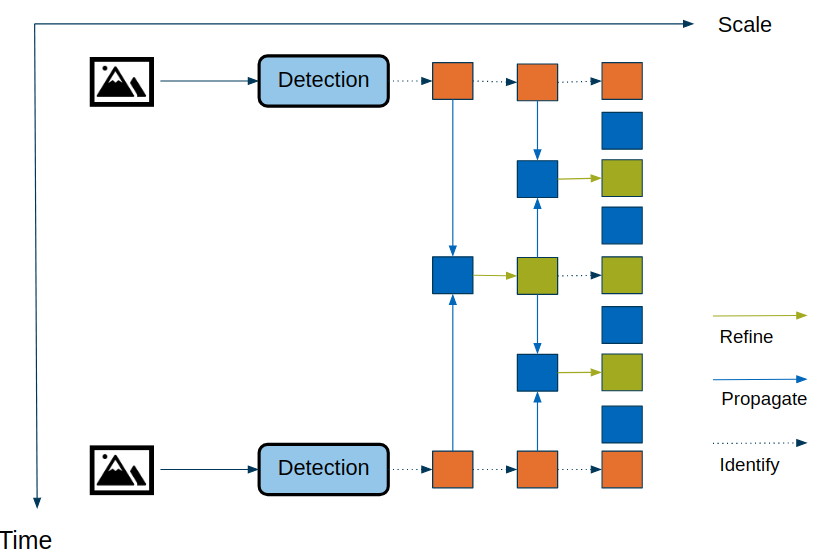
\includegraphics[width=\columnwidth]{scale-time-lattice}
\begin{itemize}
	\item Apply object detection on keyframes extracted adaptively.
	\begin{itemize}
		\item The extraction policy is based on number of objects and amount of movement in frames.
		\item If higher number/movement of objects in frames then higher extraction rate.
	\end{itemize}
	\item Propagation and refinement unit, propagates the frames temporally and refines spatially.
	\item For temporal propagation, use a small network such as resnet-18 to extract box features and a regressor to predict object movement from t to t + T.
	\item For spatial refinement, use a regressor to refine the bounding boxes over increasing scale.

\end{itemize}

\subsection{Context Matters: Refining Object Detection in Video with Recurrent Neural Networks}
Tripathi, Lipton, Belongie, Nguyen come up with a neural network architecture for video-based object detection. Their architecture consists two parts: A pseudo-labeler, which assigns labels to all video frames and a recurrent unit which refines those pseudo-labels by using the contextual information. Moreover, they describe a training strategy for their architecture and compare their approach to other models on the YouTube-Objects dataset. \newline

The final architecture can be found in \textbf{Fig 2}. Tripathi, Lipton and Belongie first train the pseudo-labeler, which is an YOLO object detection network originally trained for 20-class PASCAL VOC on the YouTube-Video Dataset. As specified in YOLO [] they minimize the weighted squared detection loss and optimize classification and localization error simultaneously. \newline

After training the pseudo-labeler they train the Recurrent Neural Network, which takes as an input the pseudo-labels and outputs improved prediction. The RNN consists of two GRU layers. \newline

For training the whole network they use the following loss function to take both accuracy at the target frame and consistency of predictions across adjacent time steps into consideration: \newline

$ loss = d_{loss} + \alpha \cdot s_{loss} + \beta \cdot c_{loss} + \gamma \cdot pc_{loss} $ \newline

For the final output Tripathi, Lipton, Belongie and Nguygen use the object detection loss as described in YOLO []:

\textbf{ToDo}

The similarity loss considers the dissimilarity between the pseudo-labels and prediction at each frame t:

\textbf{ToDo}

The category loss takes wrong class probabilities into consideration:  

\textbf{•}

And the prediction-consistency loss regularizes the model by encouraging smoothness predictions across the time-steps:

\textbf{•}

During the evaluation they find two possible areas of improvement for their approach. On the one hand the RNN is not able to recover from wrong predictions made by the pseudo-labeler after they have been fed into the RNN.  On the other hand, they observe that their network is not robust to motion. 

\subsection{Spatially Supervised Recurrent Convolutional Neural Networks for Visual Object Tracking}
In [] 

\section{Flow-based Object Detection}

\subsection{Definition}
Another type  of architectures for Video Object Detection defined, for example in [], are architectures which use Flow-Networks to consider the temporal context. The flow network estimates the optical flow which means it projects back the location in the current frame to an earlier frame. 

\subsection{Deep Feature Flow for Video Recognition}
Ning, Zhang, Huang, He, Ren and Wang design in [] a combination of box-level and feature-level based Video detectors. They use the YOLO network to create high-level visual features and preliminary location inferences and feed both into a recurrent unit. The architecture, called ROLO, is shown in \textbf{figure} \newline

They use three phases to train their model: The pre-training phase of the convolutional layers for feature learning, the traditional YOLO training phase for object proposal and the LSTM training phase for object tracking.  \newline

In the pre-training phase the convolutional layers, which create the feature maps are training on ImageNet data. Afterwards the YOLO-architecture is adopted as detection module. At least they add LSTMs for tracking. The LSTMs are fed with, the feature representations from the convolutional layers, the Bounding boxes from the detection module and the output states from the LSTM in the previous time-step. For training they use the Mean Squared Error (MSE): \newline

$ L_{MSE} = \dfrac{1}{n} TODO $ \newline

As an alternative, Ning, Zhang, Huang, He, Ren and Wang mention a Heatmap as  input for the LSTM. Therefor the prediction and the visual features are concatenated before adding them to the LSTM. This is helpful to visualize the intermediate results. \newline

Special to this architecture is, that LSTM does regression in two folds. There is a regression within one frame between the location inferences and the high-level features and there is also regression over the different frames of the sequence. 


\section{Comparison of different approaches}

\subsection{General}
\captionof{table}{Results on KITTI Dataset} 
\begin{tabular}{ | p{2cm} | p{2em}| p{2em} | p{4em} | p{5em} | } 
 \hline
 Model & MAP & FPS & Machine & Architecture \\
 \hline
 Recurrent \cite{b1} & 86.0 & 50 & Nvidia TITAN X & Feature-Level \\
 \hline
 Feature Selective \cite{b6} & 81.3 & 30.8 & Nvidia TITAN X & Feature-Level \\
 \hline
\end{tabular}

\captionof{table}{Results on ImageNet Dataset} 
\begin{tabular}{ | p{2cm} | p{2em}| p{2em} | p{4em} | p{5em} | } 
 \hline
 Model & MAP & FPS & Machine & Architecture \\
 \hline
 DT \cite{b8} & 82.0 & 7 & Nvidia TITAN X & Feature-Level \\
 \hline
 DT \cite{b8} & 78.5 & 55 & Nvidia TITAN X & Feature-Level \\
 \hline
 Scale-Time Lattice \cite{b10} & 79.6 & 20 & Nvidia TITAN X & Box-Level \\
 \hline
 Scale-Time Lattice \cite{b10} & 79 & 62 & Nvidia TITAN X & Box-Level \\
 \hline
 DeepFeature Flow \cite{b3} & 73.9 & 3 & - & Flow-Based \\
 \hline
 DeepFeature Flow \cite{b3} & 73.1 & 20.5 & - & Flow-Based \\
 \hline
 Looking Fast and Slow \cite{b7} & 60.7 & 48.8 & Pixel Phone & Feature-Level \\
 \hline
 Object Detection with Temporally-Aware \cite{b2} & 54.4 & 15 & Pixel Phone & Feature-Level \\
 \hline
\end{tabular}

\captionof{table}{Results on COCO Dataset} 
\begin{tabular}{ | p{2cm} | p{2em}| p{2em} | p{4em} | p{5em} | } 
 \hline
 Model & MAP & FPS & Machine & Architecture \\
 \hline
 Feature Selective \cite{b6} & 57.8 & 37.5 & Nvidia TITAN X & Feature-Level \\
 \hline
\end{tabular}

\captionof{table}{Results on YT Dataset} 
\begin{tabular}{ | p{2cm} | p{2em}| p{2em} | p{4em} | p{5em} | } 
 \hline
 Model & MAP & FPS & Machine & Architecture \\
 \hline
 Context Matters \cite{b4} & 68.73 & - & - & Box-Level \\
 \hline
\end{tabular}

\captionof{table}{Results on OTB Challenge Dataset} 
\begin{tabular}{ | p{2cm} | p{3em}| p{2em} | p{4em} | p{4em} | } 
 \hline
 Model & Success Rate & IoU & FPS & Machine \\
 \hline
 Spatially Supervised \cite{b5} & 0.564 & 0.455 & 20/60 & Nvidia TITAN X \\
 \hline
\end{tabular}
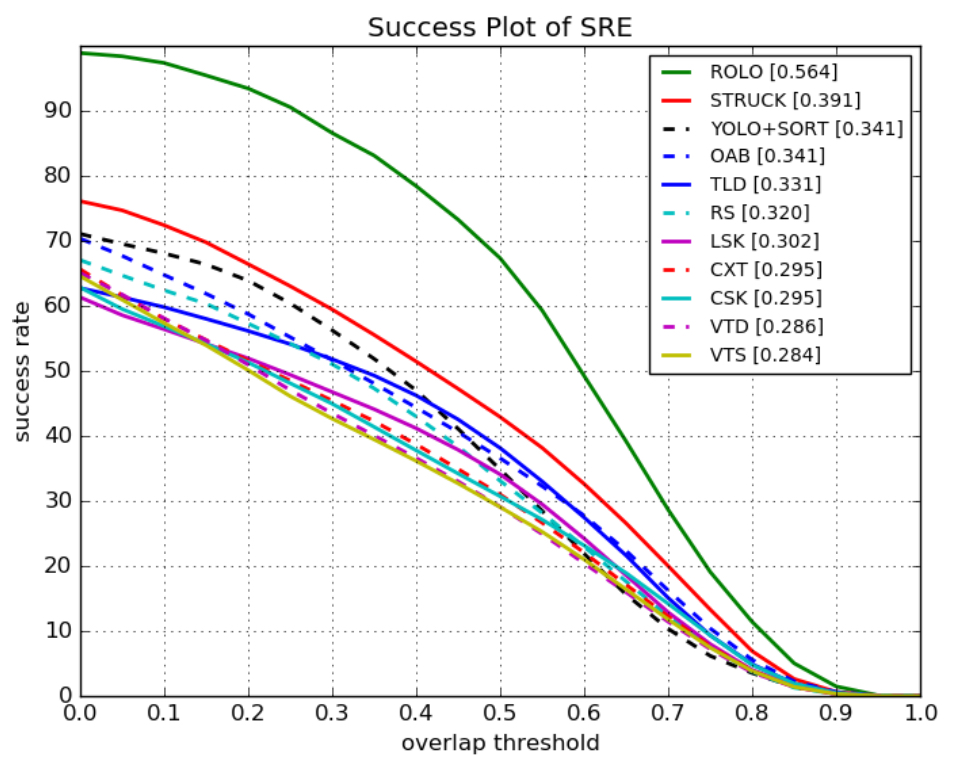
\includegraphics[width=\columnwidth]{otb-challenge-results}

\subsection{Conclusion Perfomance}
Todo

\subsection{Conclusion Prediction Quality}
Todo


\section{Outro}

\subsection{Conclusion}
Todo

\subsection{Further work}
Todo


\section*{Acknowledgment}
Todo

\section*{References}

Please number citations consecutively within brackets \cite{b1}. The 
sentence punctuation follows the bracket \cite{b2}. Refer simply to the reference 
number, as in \cite{b3}---do not use ``Ref. \cite{b3}'' or ``reference \cite{b3}'' except at 
the beginning of a sentence: ``Reference \cite{b3} was the first $\ldots$''

Number footnotes separately in superscripts. Place the actual footnote at 
the bottom of the column in which it was cited. Do not put footnotes in the 
abstract or reference list. Use letters for table footnotes.

Unless there are six authors or more give all authors' names; do not use 
``et al.''. Papers that have not been published, even if they have been 
submitted for publication, should be cited as ``unpublished'' \cite{b4}. Papers 
that have been accepted for publication should be cited as ``in press'' \cite{b5}. 
Capitalize only the first word in a paper title, except for proper nouns and 
element symbols.

For papers published in translation journals, please give the English 
citation first, followed by the original foreign-language citation \cite{b6}.

\begin{thebibliography}{00}
\bibitem{b1} Alexander Broad, Michael Jones, Teng-Yok Lee. Recurrent Multi-frame Single Shot Detector for Video Object Detection. 2018.
\bibitem{b2} Mason Liu, Menglong Zhu. Mobile Video Object Detection with Temporally-Aware Feature Maps. 2018.
\bibitem{b3} Xizhou Zhu, Yuwen Xiong, Jifeng Dai, Lu Yuan, Yichen Wei. Deep Feature Flow for Video Recognition. 2017.
\bibitem{b4} Subarna Tripathi, Zachary C. Lipton, Serge Belongie, Truong Nguyen. Context Matters: Refining Object Detection in Video with Recurrent Neural Networks.
\bibitem{b5} Guanghan Ning, Zhi Zhang, Chen Huang, Zhihai He, Xiaobo Ren, Haohong Wang. Spatially Supervised Recurrent Convolutional Neural Networks for Visual Object Tracking. 2016.
\bibitem{b6} Kai Yi, Zhiqiang Jian, Shitao Chen, Nanning Zheng. Feature Selective Small Object Detection via Knowledge-based Recurrent Attentive Neural Network. 2019.
\bibitem{b7} Mason Liu, Menglong Zhu, Marie White, Yinxiao Li, Dmitry Kalenichenko. Looking Fast and Slow: Memory-Guided Mobile Video Object Detection. 2019.
\bibitem{b8} Christoph Feichtenhofer, Axel Pinz, Andrew Zisserman. Detect to Track and Track to Detect. 2017.
\bibitem{b9} Kai Kang, Wanli Ouyang, Hongsheng Li, Xiaogang Wang. Object Detection from Video Tubelets with Convolutional Neural Networks. 2016.
\bibitem{b10} Kai Chen, Jiaqi Wang, Shuo Yang, Xingcheng Zhang, Yuanjun Xiong, Chen Change Loy, Dahua Lin. Optimizing Video Object Detection via a Scale-Time Lattice. 2018.
\bibitem{b11} Ian Goodfellow, Yoshua Bengio, Aaron Courville. Deep Learning (Adaptive Computation and Machine Learning). 2017.
\bibitem{b12} Alexander Broad, Michael Jones, Teng-Yok Lee. Supplementary Material for Recurrent Multi-frame Single Shot Detector for Video Object Detection. 2018.
\bibitem{b13} Jia Deng, Wei Dong, Richard Socher, Li-Jia Li, Kai Li and Li Fei-Fei. ImageNet: A Large-Scale Hierarchical Image Database. 
\bibitem{b14} Alex Krizhevsky, Ilya Sutskever, Geoffrey E. Hinton. ImageNet Classification with Deep Convolutional Neural Networks. 2012.
\bibitem{b15} Shaoqing Ren, Kaiming He, Ross Girshick, Jian Sun. Faster R-CNN: Towards Real-Time Object Detection with Region Proposal Networks. 2016. 
\bibitem{b16} Joseph Redmon, Ali Farhadi. YOLOv3: An Incremental Improvement.
\bibitem{b17} Wei Liu, Dragomir Anguelov, Dumitru Erhan, Christian Szegedy, Scott Reed, Cheng-Yang Fu, Alexander C. Berg. SSD: Single Shot MultiBox Detector. 2016.
\end{thebibliography}
\vspace{12pt}

\end{document}
